\documentclass[conference]{IEEEtran}
\usepackage{times}
\usepackage{graphicx}
\usepackage{booktabs}
\usepackage{subfigure}
\usepackage{latexsym,amssymb,amsmath} % for \Box, \mathbb, split, etc.
%\usepackage{path}
\usepackage{url}
\usepackage{verbatim}
\usepackage[numbers]{natbib}
\usepackage{amsfonts}
\usepackage{color}
\usepackage{hyperref}
\hypersetup{letterpaper,bookmarksopen,bookmarksnumbered,
pdfpagemode=UseOutlines,
colorlinks=true,
linkcolor=blue,
anchorcolor=blue,
citecolor=blue,
filecolor=blue,
menucolor=blue,
urlcolor=blue
}

\newcommand{\stnote}[1]{\textcolor{blue}{\textbf{ST: #1}}}
\newcommand{\jgonote}[1]{\textcolor{green}{\textbf{JGO: #1}}}

\usepackage{algorithmic}


\newcommand{\mytitle}[0]{Autonomously Acquiring Models of Objects for
  Instance-Based Manipulation}

\pdfinfo{
   /Author ()
   /Title  (\mytitle)
   /CreationDate (D:20101201120000)
   /Subject (Robots)
   /Keywords ()
}



\makeatletter
\setlength{\arraycolsep}{2\p@} % make spaces around "=" in eqnarray smaller
\makeatother


% begin of personal macros
\newcommand{\half}{{\textstyle \frac{1}{2}}}
\newcommand{\eps}{\varepsilon}
\newcommand{\myth}{\vartheta}
\newcommand{\myphi}{\varphi}

\newcommand{\IN}{\mathbb{N}}
\newcommand{\IZ}{\mathbb{Z}}
\newcommand{\IQ}{\mathbb{Q}}
\newcommand{\IR}{\mathbb{R}}
\newcommand{\IC}{\mathbb{C}}
\newcommand{\Real}[1]{\mathrm{Re}\left({#1}\right)}
\newcommand{\Imag}[1]{\mathrm{Im}\left({#1}\right)}

\newcommand{\norm}[2]{\|{#1}\|_{{}_{#2}}}
\newcommand{\abs}[1]{\left|{#1}\right|}
\newcommand{\ip}[2]{\left\langle {#1}, {#2} \right\rangle}
\newcommand{\der}[2]{\frac{\partial {#1}}{\partial {#2}}}
\newcommand{\dder}[2]{\frac{\partial^2 {#1}}{\partial {#2}^2}}

\newcommand{\nn}{\mathbf{n}}
\newcommand{\xx}{\mathbf{x}}
\newcommand{\uu}{\mathbf{u}}

\newcommand{\junk}[1]{{}}

% set two lengths for the includegraphics commands used to import the plots:
\newlength{\fwtwo} \setlength{\fwtwo}{0.45\textwidth}


%% \renewcommand{\labelitemi}{}
%% \renewcommand{\labelitemii}{}
%% \renewcommand{\labelitemiii}{}


% end of personal macros
% \input{inputFile.tex}


\begin{document}
%\DeclareGraphicsExtensions{.jpg}


\title{\mytitle{}}

\author{Author Names Omitted for Anonymous Review. Paper-ID [add your ID here]}

\maketitle


%% To address this problem, we define a SLAM-based approach
%% which enables the robot to actively acquire visual and grasp models of
%% novel objects by moving its sensor and trying grasps, integrating
%% information over time.  Unlike conventional SLAM, in our model the
%% hidden state is the object pose, and the map consists of invariant
%% features of the object such as appearance information and grasp
%% points.  

\begin{abstract}
Manipulating and reasoning about objects is an important task for
robots that help people in the home, in factories, and in hospitals.
A key aim of current research is to create robots that can reliably
manipulate generic objects in clutter.  However in many applications,
general-purpose object detection or manipulation is not required: the
robot would be useful if it could recognize, localize, and manipulate
the relatively small set of specific objects most important in that
application, but do so with very high reliability.  To address this
problem, we focus not on {\em category-based} manipulation (pick up
any mug) but rather {\em instance-based} manipulation (pick up this
mug).  Instance-based recognition and pose estimation using vision can
be highly accurate but requires adapting the system to the specific
object being manipulated: the system designer must adapt the system to
specific objects in the environment in large and small ways, ranging
from collecting training data to choosing parameter values to
selecting algorithms for tasks such as image segmentation or bounding
box classification.  The contribution of this paper is to formalize
this adaptation process as a hierarchy of bandit problems, enabling
the robot to apply learning techniques such as Thompson sampling to
learn to manipulate specific objects.  Our framework runs on an
unmodified Baxter robot; using our algorithm, a robot can interact
with an object for twenty minutes, and then reliably and quickly
localize it with vision and pick it up with closed-loop visual
servoing. We demonstrate that the adaptation step significantly
improves accuracy over a non-adaptive system.


%% Robots need to pick stuff up.
%% %
%% Perception can structure data, structured data facilitates planning, planning allows more principled perception.
%% %
%% The tasks of robotic perception, planning, and control will all benefit from
%% a design paradigm which allows them to be jointly programmed.
%% %
%% So we contribute an implementation \emph{NODE} which facilitates the design and 
%% execution of versatile and scalable MDPs structured in what we call a
%% Von Neumann MDP pattern. 
%% %
%% We form a closed loop through perception and planning, allowing them to interact by means of structured data.
%% %
%% Our system incorporates online, human-in-the-loop algorithms. Non-technical human participants can easily
%% teach and collaborate with the system.
\end{abstract}


% First paragraph: What is the problem we are trying to solve? I
% think it's something about enabling a robot to robustly perceive and
% manipulate native objects, so that it can carry out tasks such as
% assisting at childcare, cooking, or in hospitals.
% Second paragraph: Why hasn't previous work addressed this problem?
% I think it's something about the focus on category recognition, not
% doing pose estimation, and training methods that require an expert
% user and an annotated corpus.
% Third paragraph: What do we propose to do to address this problem?
% Fourth paragraph: Our high-level technical approach
% Fifth paragraph: How do we know it works? Why is it cool?
% Something about an evaluation and something about a robotic
% demonstration.

\section{Introduction}
Robotic assistants will assist us at childcare, help us cook, and
provide service to doctors, nurses, and patients in hospitals. Many of
these tasks require a robot to robustly perceive and manipulate
objects in its environment, yet robust object manipulation remains a
challenging problem.  Systems for general-purpose manipulation are
computationally expensive and do not enjoy high accuracy on novel
objects~\citep{saxena08}.  Instance-based approaches that focus on
specific instances of objects can have higher accuracy but require
training by a human operator, which is time consuming and can be
difficult for a non-expert to perform ~\citep{ork14, lai11, lai11a}.
Existing approaches to autonomously learn 3d object models still
require expensive ICP-based methods to localize objects, which are
susceptible to local minima and take time to
converge~\citep{krainin11}.

Instead we propose an approach that enables a robot to autonomously
learn a view-based model for closed-loop visual picking.  View-based
methods for instance detection have many advantages over methods using
3d models, because they directly capture the visual appearance of the
object, and are relatively simple and efficient to implement because
they operate on low-level features~\citep{hsiao13}.  However these
systems require large amounts of training data for robust performance,
for example more than 2000 images which must be manually collected and
annotated with bounding boxes for the state of the art LINE2D
method~\citep{hinterstoisser12}.  Moreover, for manipulation,
view-based methods do not propose potential grasps, and autonomous
methods for recognizing visual grasps are prone to error. 

We address this problem by enabling a robot to learn to identify and
grasp on a per object basis by autonomously collecting large amounts
of data for instance-based visual detection and pose estimation.  We
formalize a general algorithm for closed-loop picking with active
servoing.  This pipeline uses standard computer vision techniques and
is not itself novel.  Our contribution is a formalization of this
pipeline together with reward signals for each module. This
formalization enables the robot to use a bandit-based algorithm to
autonomously and actively train its subsystems for specific objects.
We use slower, more accurate sensing approaches to provide supervision
for faster, simpler methods that excel with large amounts of training
data.  For example, to perform grasping we use an analytic model to
select grasp points, but depending on the object, the best grasp
according to the analytic model may not be optimal; the robot can
learn better grasps for that object using the analytic model as a
prior and actively collecting data for that object.

%% To address these issues, we present an approach for enabling a robot
%% to train its own view-based model to recognize and manipulate the
%% specific objects it will need to use during collaborations with
%% humans.  Using our algorithm, the robot detects candidate objects for
%% training using a depth sensor, then actively collects view-based
%% visual templates to perform robust instance-based object detection,
%% pose estimation and closed-loop grasping using visual servoing.
%% Because our camera can move with seven degrees of freedom, the robot
%% can collect large quantities of data leading to simple visual models
%% that perform with high accuracy even under occlusion.  Our approach is
%% enabled by three innovations: our end-to-end algorithm for collecting
%% view-based training data with supervision obtained from a
%% higher-reliability depth sensor, which is supported by a simple and
%% robust method for determining candidate grasps using a depth sensor
%% mounted on a seven-degree-of-freedom arm, along with an approach for
%% autonomously and reliably finding object bounding boxes once the
%% object is on a background such as a floor or table.

Our evaluation demonstrates that a Baxter robot can autonomously learn
robust models for detection and grasping, using its IR sensor and arm
camera as a seven-degree of freedom one-pixel RGB-D camera.  After
training, Baxter can quickly and reliably grasp objects anywhere in
its work space using closed-loop visual servoing in response to a
person's requests.  We demonstrate that our baseline system can learn
to pick up objects approximately 50\% of the time; augmenting this
system with our self-training approach increases accuracy to XX\%.

%% Our software is compatible with ROS and the Baxter SDK version 1.0.0,
%% and we intend to release it as free software should our paper be
%% accepted.  Our software includes the capability to upload
%% instance-based models to the RoboBrain database~\citep{x}; as more and
%% more instance-based models are collected, this corpus will form a
%% unique training set for category-based models for detecting and
%% grasping novel objects, since the robot will have a very large number
%% of views of a large set of objects as well as storing depth
%% information and grasping success.


\section{Grasping System}

We first describe our instance-based object detection and pose
estimation pipeline, which uses standard computer vision algorithms
combined to achieve a simple software architecture, a high frame rate,
and high accuracy at recognition and pose estimation.  This pipeline
can be manually trained by an expert to reliably detect and grasp
objects.  Section~\ref{sec:training} describes our approach to
enabling a robot to autonomously train this pipeline by actively
collecting images and training data from the environment using
Thompson sampling.

Our recognition pipeline takes video from the robot, proposes a small
number of candidate object bounding boxes in each frame, and
classifies each candidate bounding box as belonging to a previously
encountered object class. Our object classes consist of object
instances rather than pure object categories.  Using instance
recognition means we cannot reliably detect categories, such as
``mugs,'' but the system will be able to detect, localize, and grasp
the specific instances for which it has models with much higher speed
and accuracy.  A visualization of data flow in the pipeline appears in
Figure~\ref{fig:system}.  For each module, we formalize its input,
output, and reward function; each component can have multiple
implementations which better for different objects.  The following
sections describe how we can use this pipeline to learn which
implementation to use for specific objects; this learning dramatically
speeds up performance.

\begin{figure}
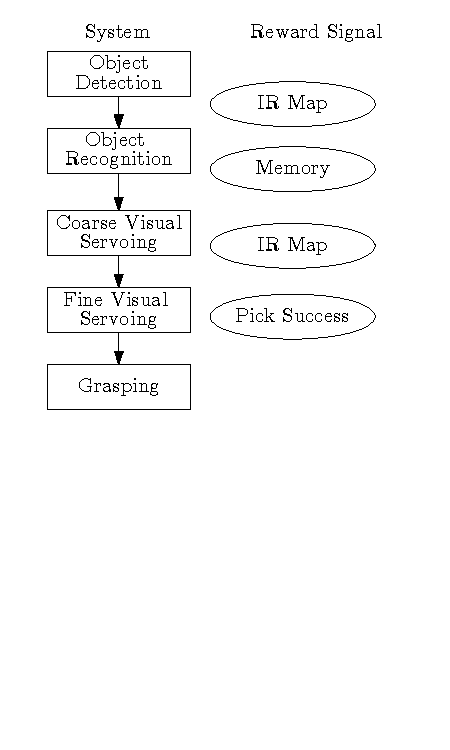
\includegraphics{system.pdf}
\caption{Data flow in our grasping system.\label{fig:system}}
\end{figure}

\subsection{Object Detection}
\label{sec:detection}

The input of the object detection component is an image, $I$; the
output is a set of candidate bounding boxes, $B$.  We validate this
component during training using the 3d IR map of the object, which we
back-project into the original image to obtain the true bounding box.
We use two algorithms for object detection, one based on the BING
objectness metric, which works well for objects that have distinct
colors, and one based on gradients, which works well for objects that
contrast well with the background. 

\subsubsection{Detecting Objects Using BING and Integral Images}

To detect candidate objects, we first apply the BING objectness
detector~\citep{cheng14} to the image, which returns a set $\{B_i\}$
of thousands of approximate object bounding boxes in the image, shown
in Figure~\ref{fig:bing}. This process substantially reduces the
number of bounding boxes we need to consider but is still too large to
process in real time. Besides, even good bounding boxes from BING are
typically not aligned to the degree that we require. Therefore, we use
integral images to efficiently compute the per-pixel map:
\begin{align}
J(p) = \sum_{B \in \{B_i\} s.t. p \in B} \frac{1}{Area(B)}.
\end{align}

This map appears in Figure~\ref{fig:objectness}.  We then apply the
Canny edge detector with hysteresis ~\citep{canny86} to find the
connected components of bright regions in the map $J(p)$, which
correspond with high probability to objects in the image. We form our
candidate object bounding boxes by taking the smallest bounding box
which surrounds each connected component, shown in
Figure~\ref{fig:bounding_boxes}.  These bounding boxes make it easy to
gather training data and to perform inference in real time, but at the
expense of poorly handing occulusion as overlapping objects are fused
into the same bounding box.  It is possible to search within the
proposed bounding boxes to better handle occlusion.
Figure~\ref{fig:object_detection} shows images from each step in this
pipeline, ending with just one candidate bounding boxes for an objects
on an empty table.  Note that we designed this pipeline to quickly and
accurately provide bounding boxes in the presence of relatively
unobstructed backgrounds to support the training process;
Section~\ref{sec:mapping} describes our approach to recognition under
clutter and occlusion.

\subsubsection{Detecting Objects Using Image Gradients}

\stnote{John -- please fill this part in.}

\subsection{Object Recognition}
\label{sec:recognition}

The object recognition module takes as input a bonding box, $B$, and
outputs a label for that object, $c$, based on the robot's memory.
This label is used to identify the object and look up other
information about the object for grasping further down the pipeline.

For each object $c$ we wish to classify, we gather a set of example
crops $E_c$ which are candidate bounding boxes (derived as above)
which contain $c$. We extract dense SIFT features ~\citep{lowe99} from
all boxes of all classes and use k-means to extract a visual
vocabulary of SIFT features ~\citep{szeliski10}. We then construct a
BoW feature vector for each image and augment it with a histogram of
colors which appear in that image.  The augmented feature vector is
incorporated into a k-nearest-neighbors model which we use to classify
objects at inference~\citep{szeliski10}. We use kNN because our
automated training process allows us to acquire as much high-quality
data as necessary to make the model work well, and kNN supports direct
matching to this large dataset.  Existing approaches for
instance-based grasping such as LINE-2D require the order of $2000$
whereas our SIFT-based approach performs well with only $200$
examples~\citep{hinterstoisser12}.


%% The use of SIFT features is motivated by the instance level nature of
%% our task. State-of-the-art vision methods typically use
%% HOG~\citep{dalal05} features, but that choice is motivated by category
%% level recognition. \stnote{What about category level recognition
%%   motivates HOG or CNN?  Can you be more specific?}


%% is easy to rebuild online, which is a key
%% property a classifier should enjoy if it is to interact with our
%% framework in real time. State-of-the-art computer vision classifiers
%% currently employ SVM's ~\citep{} or other models which require
%% expensive training. Using such a model would introduce a training step
%% in the inside loop of our data collection process, which would be
%% costly in either engineering or time.  It is possible to use kNN
%% during the online collection process and then train a stronger
%% classifier in the background at higher latency, essentially
%% introducing a cascading step in the data collection process.

\begin{figure*}
\subfigure[Raw image from the camera.]{
  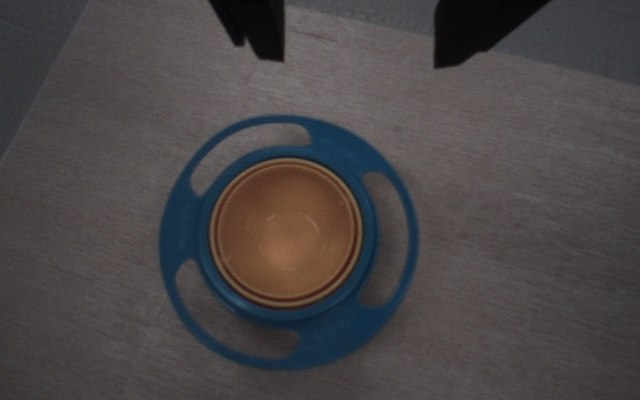
\includegraphics[width=0.25\linewidth]{figures/objectness_raw.png}}%
\subfigure[Candidate bounding boxes from Bing.\label{fig:bing}]{
  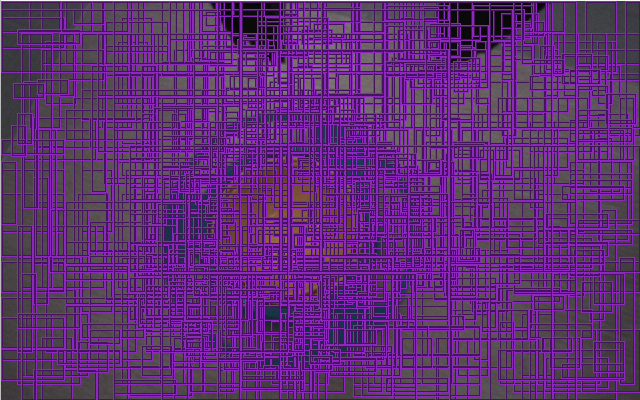
\includegraphics[width=0.25\linewidth]{figures/objectness_purple.png}}%
\subfigure[Integral image objectness map.\label{fig:objectness}]{
  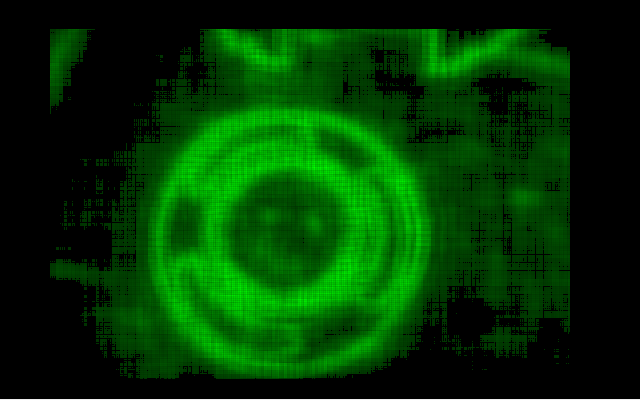
\includegraphics[width=0.25\linewidth]{figures/objectness_map.png}}%
\subfigure[Candidate bounding boxes.\label{fig:bounding_boxes}]{
  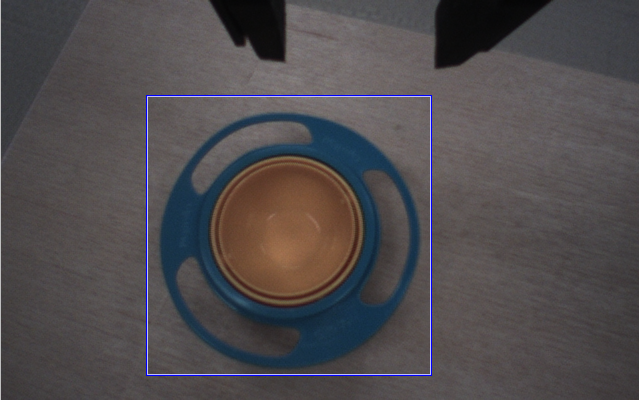
\includegraphics[width=0.25\linewidth]{figures/objectness_boxes1.png}}
\caption{The object detection pipeline, showing a raw image from the
  camera, the integral image computed using objectness, and candidate
  bounding boxes.\label{fig:object_detection}}
\end{figure*}



 
\subsection{Pose Estimation}

To perform pose estimation, we require an image gradient of the object
at a specific, known pose:

\begin{align}
\Delta I = \left( \frac{\partial I}{\partial x}, \frac{\partial I}{\partial y} \right)
\end{align}

We approximate the gradiant using differences after smoothing the
training image:
\begin{align}
\frac{\partial I(x, y)}{\partial x} \approx \frac{I(x + 1, y) - I(x - 1, y)}{2}\\
\frac{\partial I(x, y)}{\partial y} \approx \frac{I(x, y + 1) - I(x, y - 1)}{2}
\end{align}

To estimate pose, we perform data augmentation by rotating our
training image and finding the closest match to the image currently
recorded from the camera, as detected and localized via the pipeline
in Section~\ref{sec:detection} and~\ref{sec:recognition}.

\subsection{Identifying Grasp Points}

To identify a grasp points, we combine a depth map of the object with
a model of the gripper.  The depth map appears in
Figure~\ref{fig:depth_map}.  The grasp model scores each potential
grasp according to a linear model of the gripper to estimate grasp
success.  A default algorithm picks the highest-scoring grasp point,
but frequently this point is not actually a good grasp, because the
object might slip out of the robot's gripper or part of the object may
not be visible in IR.  The input to this module is the 3d pose of the
object, and the output is a grasp point $(x, y)$; at this point we
assume only crane grasps rather than full 3d grasping. 



\subsection{Closed-Loop Grasping}

To grasp an object, we first scan the work area by moving the camera
until the object is detected an recognized.  Then we perform active
visual servoign to move the arm directly above the object.  Next, we
perform orientation servoing using the pose estimation
algorithm. Because these components are instance-based, they report
position and orientation with high accuracy, enabling us to use a
proportional controller (with no derivative or integral terms) to move
the arm into





\section{Autonomous Training}
\label{sec:training}

An object model in our framework consists of the following elements:
\begin{itemize}
\item cropped object templates (roughly 200), $t^1 ... t^K$
\item depth map, $D$, which consists of a point cloud, $(x, y, z, r, g, b, d)$.
\item cropped gradient template, $t_0$
\end{itemize}

Additionally, the model can be augmented with words or attributes,
$w_1... w_n$ which people might use to describe the object, so the
robot can respond to natural language commands such as ``Put the cup
on the left table.''

To train our model, the robot first moves the object to a known pose,
then acquires images that are annotated with a pose as well as a
cropped bounding box for training.  As typical in machine learning
applications, the more images we can acquire, from the more
viewpoints, the more accurate our detection, pose estimation, and
grasping.  To achieve this accuracy, the robot autonomously collects
this information by using a depth sensor to acquire an initial grasp,
move the object to a standard known pose, and then actively collect
data for view-based methods.  Our learning algorithm appears in
Algorithm~\ref{alg:learning}.

Once the object has been moved to a known pose, we acquire the object
model by moving the camera to a sequence of prespecified orientations.
We automatically crop the image using integral images computed over
the bounding boxes inferred by the Bing objectness detector.


\begin{figure}
  \textbf{GraspObject()}
  \begin{algorithmic}
    \WHILE {true}
      \STATE $I \gets loadImage()$
      \STATE $B \gets Attempt a grasp.$
      \IF {grasp is successful}
        \STATE Move object to training area.
        \STATE Map(object).
      \ENDIF
    \ENDWHILE
  \end{algorithmic}
  \caption{The high-level object-learning algorithm.\label{alg:learning}}
\end{figure}


\begin{figure}
  \textbf{Map}
  \begin{algorithmic}
    \FOR {$(x^k, y^k, z^k) \in scan$}
    \STATE $I^k \gets ImageAt (x^k, y^k, z^k)$
    \STATE $t^k \gets Crop(I^k)$ using the approach described in Section~\ref{sec:detection}
    \STATE $D^k \gets PointAt(x^k, y^k, z^k)$
    \ENDFOR
  \end{algorithmic}
  \caption{The high-level algorithm for acquiring visual and grasping
    models of objects.}
\end{figure}


\section{Bandit-based Adaptation}

 
\section{Experimental Setup}

The aim of our evaluation is to assess the ability of the system to
acquire visual models of objects which are effective for grasping and
object detection.  We have implemented our approach on the Baxter
robot, which is equipped with a seven-degree-of-freedom arm with a
camera and IR depth sensor, which we use as a one-pixel depth camera
to acquire our models.

\subsection{Object Detection and Pose Estimation}

For object Detection and pose estimation, we constructed data sets on
which we could evaluate our models. This involved hand annotating the
ground truth for the images in the sets, which is a costly procedure
which we are attempting to eliminate for future tasks.  However, we
cannot evaluate our system in a principled fashion without such a data
set.

We demonstrate our method's success in this setting where we pay the cost
to acquire the data so that we can trust our method and that cost need not be 
payed during future applications. 

Probably uses confusion rates as the objective function.

Expert viewpoint collection (uses at least hard negatives)

Super dense sampling

uniform hard negative sampling with stopping criterion



\section{Evaluation and Discussion}

We could report the performance of the system as a function of user
interactions.  We could report the performance of the system as a
function of program lifetime.  Our representative set could consist of
a block, a spoon, a bowl, a diaper, and a sippy cup. A \emph{single
  cut video} showing multiple grasps of all objects is available here.

\subsection{Object Detection}

We establish a baseline for performance by training the system in a
representative domain specific setting, which tells us how well it can
perform on laboratory objects when trained by an expert. This
represents the best that the system could be expected to perform.

\begin{table}
  \begin{center}
  \caption{Performance of our system on the object detection task.}
  \begin{tabular}{lr}
    \toprule
  Data Collection Method & Success Rate \\ 
  \midrule
  Expert Annotation & 0.0 \\ 
  Dense Sampling & 0.0 \\ 
  Hard Negatives Auto-Stopping & 0.0 \\ 
  \bottomrule
  \end{tabular}
  \end{center}
\end{table}

\subsection{Pose Estimation}

\begin{table}
  \caption{Performance of our system on offline data.}
  \begin{center}
  \begin{tabular}{lr}
\toprule
  Data Set            &  \\ 
\midrule
  Expert Curated      & 0.0 \\ 
  Expert (noisy)      & 0.0 \\ 
  Automatic (curated) & 0.0 \\ 
  Automatic (noisy)   & 0.0\\
\bottomrule
  \end{tabular}

  \end{center}
\end{table}


\subsection{Grasping}

\begin{figure}
  \begin{center}
  \begin{tabular}{lr}
  \toprule
  Grasp Sampling Method & Success Rate \\ 
  \midrule
  Expert Annotation & 0.0 \\ 
  Uniform Sampling & 0.0 \\ 
  Thompson Sampling & 0.0 \\
  \bottomrule
  \end{tabular}
  \caption{Performance of our system on the grasping task.}
  \end{center}
\end{figure}

\subsection{PID Control}

\begin{figure}
  \begin{center}
  \begin{tabular}{lr}
    \toprule
  Parameter Learning Method & Average Convergence Time \\ 
  \midrule
  Expert Annotation & 0.0 \\ 
  Constant Learning Rate & 0.0 \\
  Decaying Learning Rate & 0.0 \\
  Wide Scale Random Noise & 0.0 \\
  \bottomrule
  \end{tabular}
  \caption{Performance of our system on the PID control task.}
  \end{center}
\end{figure}

%\subsection{Laboratory Automatic Training}
%How well does the automatic training system perform when trained in laboratory conditions?

%\subsection{Non-Expert In-The-Wild Training}
%We then go on to compare the performance of the system when trained to various degrees by naive
%and technical non-expert users.
%We repeat the experiments with naive users in two settings. In the first, they train laboratory
%objects. In the second, they provide their own objects.


\section{Related Work}

\citet{bohg13} survey data-driven approaches to grasping.  Our
approaches can be thought of as a pipeline for automatically building
an experience database consisting of object models and known good
grasps, using analytic approaches to grasping unknown objects to
generate a grasp hypothesis space and bandit-based methods for trying
grasps and learning instance-based distributions for the grasp
experience database.  In this way our system achieves the best of both
approaches: models for grasping unknown objects can be applied; when
they do not fail, the system can automatically recover by trying
grasps and adapting itself based on that specific object. 

\citet{ude12} described an approach for detecting and manipulating
objects to learn models.  It uses a bag of words model and learns to
detect the objects.  It does not learn a model for grapsing.
\citet{schiebener13} describes an extension that also does model
learning.  The robot pushes the object and then trains an object
recognition system.  It does nto use a camera that move and does not
grasp.
\citet{schiebener12} discovers and grasps unknown objects.

Summary: 
\begin{itemize}
\item People doing SLAM.  \citet{wang07, gallagher09}, 
\item People doing 3d reconstruction.   \citet{krainin11, banta00}
\item People doing big databases for category recognition.  \citet{kent14a, kent14, lai11a, goldfeder09}
\item Object tracking in vision (typically surveillance).
\item POMDPs for grasping.  \citet{platt11, hsiao10}
\item People doing systems.  \citet{hudson12, ciocarlie14}
\end{itemize}




Crowd-sourced and web robotics have created large databases of objects
and grasps using human supervision on the web~\citep{kent14a, kent14}.
These approaches outperform automatically inferred grasps but still
require humans in the loop.  Our approach enables a robot to acquire a
model fully autonomously, once the object has been placed on the
table.

\citet{zhu14} created a system for detecting objects and estimating
pose from single images of cluttered objects.  They use KinectFusion
to construct 3d object models from depth measurements with a
turn-table rather than automatically acquiring models.

\citet{chang12} created a system for picking out objects from a pile
for sorting and arranging but did not learn object models.  

next-best view planning~\citep{kriegel11}

\citet{nguyen14} learn to manipulate objects such as a light switch or
drawer with a similar self-training approach.  Our work learns visual
models for objects for autonomous pick-and-place rather than to
manipulate objects.

Developmental/cognitive robotics~\citep{lyubova13, kraft10r}

\citet{banta00} constructs a prototype 3d model from a minimum number
of range images of the object.  It terminates reconstruction when it
reaches a minimum threshold of accuracy.  It uses methods based on the
occluded regions of the reconstructed surfice to decide where to place
the camera and evaluates based on the reconstruction rather than pick
up success.  \citet{krainin11} present an approach for autonomous
object modeling using a depth camera observing the robot's hand as it
moves the object.  This system provides a 3d construction of the
object autonomously.  Our approach uses vision-based features and
evaluates based on grasp success.  Eye-in-hand laser
sensor.~\citep{aeotti14}

\stnote{Need to find the instance-based work that Erik mentioned when
  he said it was a ``solved problem.''}

\citet{velez11} created a mobile robot that explores the environment
and actively plans paths to acquire views of objects such as doors.
However it uses a fixed model of the object being detected rather than
updating its model based on the data it has acquired from the
environment.

Methods for planning in information space \citep{he08, atanasov13,
  prentice09} have been applied to enable mobile robots to plan
trajectories that avoid failures due to inability to accurately
estimate positions.  Our approach is focused instead on
object detection and manipulation, actively acquiring data for use
later in localizing and picking up objects. \stnote{May need to say
  more here depending on what GRATA actually is.}


Early models for pick-and-place rely on has been studied since the
early days of robotics~\citep{brooks83, lozano89}.  These systems
relied on models of object pose and end effector pose being provided to the
algorithm, and simply planned a motion for the arm to grasp.  Modern
approaches use object recognition systems to estimate pose and object
type, then libraries of grasps either annotated or learned from
data~\citep{saxena08, goldfeder09, morales03}.  These approaches
attempt to create systems that can grasp arbitrary objects based on
learned visual features or known 3d configuration.  Collecting these
training sets is an expensive process and is not accessible to the
average user in a non-robotics setting.  If the system does not work
for the user's particular application, there is no easy way for it to
adapt or relearn.  Our approach, instead, enables the robot to
autonomously acquire more information to increase robustness at
detecting and manipulating the specific object that is important to
the user at the current moment.

Visual-servoing based methods~\citep{chaumette06} \stnote{Need a whole
  paragraph about that. }

\stnote{\citet{ciocarlie14} seems highly relevant, could not read from
  the train's wifi.}  Existing work has collected large database of
object models for pose estimation, typically curated by an
expert~\citep{lai11}.  \citet{kasper12} created a semiautomatic system
that fuses 2d and 3d data, but the setup requires a special rig
including a turntable and a pair of cameras.  Our approach requires an
active camera mounted on a robot arm, but no additional equipment, so
that a robot in the home can autonomoulsy acquire new models.

\citet{collect14} describes an approach for lifelong robotic object
discovery, which infers object candidates from the robot's perceptual
data.  This system does not learn grasping models and does not
actively acquire more data to recognize, localize, and grasp the
object with high reliabilitiy.  It could be used as a first-pass to
our system, after which the robot uses an active method to acquire
additional data enablign it to grasp the object.  Approaches that
integrate SLAM and moving object tracking estimate pose of objects
over time but have not been extended to manipulation~\citep{wang07,
  gallagher09, salas-moreno13, selvatici08}.

Our approach is similar to the philosphy adopted by Rethink Robotic's
Baxter robot, and indeed, we use Baxter as our test
platform~\citep{fitzgerald13}.  \stnote{Haven't actually read this
  paper, just making stuff up based on Rod's talks.  Should read the
  paper and confirm.}  Baxter's manufacturing platform is designed to
be easily learned and trained by workers on the factory floor.  The
difference between this system and our approach is we rely on the
robot to autonomously collect the training information it needs to
grasp the object, rather than requiring this training information to
be provided by the user.


Robot systems for cooking~\citep{bollini12, beetz11} or furniture
assembly~\citep{knepper13} use many simplifying assumptions, including
pre-trained object locations or using VICON to solve the perceptual
system.  We envision vision or RGB-D based sensors mounted on the
robot, so that a person can train a robot to recognize and manipulate
objects wherever the robot finds itself.

Approaches to plan grasps under pose uncertainty~\citep{stulp11} or
collect information from tacticle sensors~\citep{hsiao10} using
POMDPs.  \citet{plat11} describe new algorithms for solving POMDPs by
tracking belief state with a high-fidelity particle filter, but using
a lower-fidelity representation of belief for planning, and tracking
the KL divergence.

\citet{hudson12} used active perception to create a grasping system
capable of carrying out a variety of complex tasks.  Using feedback is
critical for good performance, but the model cannot adapt itself to
new objects.



\section{Conclusion}

\stnote{First paragraph:  contributions.  What are the things this paper has done to advance the state of the art?}

\stnote{Next paragraphs: future work, spiraling upward to more and
  more ambitiuos extensions.}

Right now, NODE runs on Baxter. We will port NODE to PR2 and other AH systems.
GRATA could be applied in other domains as well.  What are some examples?

Ideas for doing for the paper, otherwise future work: 
\begin{itemize}
\item Semantic mapping. 
\item Detection and manipulation in clutter and occlusion.
\item Amazon mechanical turk for labels, so we can follow commands and gesture.
\item Object tracking over time so we can answer questions about what
  happened to the object.
\item Object oriented SLAM so we can handle joint localization and mapping.
\item Semantic mapping of objects over time.  Deciding when to go look
  again, maintaining history, etc. 
\item Scaling to lots and lots of objects.
\item Using the database of lots and lots of objects to do category recognition.
\item Multiple poses during training (e.g., what happens when you drop
  the object?)
\end{itemize}

% Intro structure
% First paragraph: What is the problem we are trying to solve? 
% Second paragraph: Why hasn't previous work addressed this problem?
% Third paragraph: What do we propose to do to address this problem?
% Fourth paragraph: What is our high-level technical approach.
% Fifth paragraph: How do we know it works? Why is it cool?
%
% 1. Experimental
%  a. Contribution (Is it new?)
%  b. Execution (Does it work?)
%  c. Demonstration (Is it well understood? were the choices made well?)
% 2. Bureaucratic
%  a. Do we know what we are talking about?
%  b. CYA (Are we polite about it? Are we accidently claiming false novelty?)
%  c. Do they know what we are talking about? (No algebraic geometry plz k thnx.)
% 3. Aesthetic
%  a. Grammar and Spelling
%  b. Vocab and Word Choice
%  c. Prosody (Does it scan? How is the meter?)

\bibliographystyle{plainnat}
\bibliography{main,references}


\end{document}
